%2345678901234567890123456789012345678901234567890123456789012345678901234567890
%%%%%%%%%%%%%%%%%%%%%%%%%%%%%%%%%%%%%%%%%%%%%%%%%%%%%%%%%%%%%%%%%%%%%%%%%%%%%%%%
% MAURICIO ESGUERRA NEIRA
% Ph. D. Thesis
%%%%%%%%%%%%%%%%%%%%%%%%%%%%%%%%%%%%%%%%%%%%%%%%%%%%%%%%%%%%%%%%%%%%%%%%%%%%%%%%
\chapter{RNA Base Steps}
\label{basesteps} 
\bibliographystyle{nar}
The problem of classification of the space of conformations
%configurations?
of RNA  is not  new, see for  example, Olson  1972 \cite{olson1_1972},
Saenger     1984     \cite{saenger1984},     and    Gautheret     1993
\cite{gautheret1993}.  This  problem had only been addressed  by a few
researchers  before the  turn of  the twenty  first century,  now this
situation is changing rapidly. The reason for this fast change came in
the year 2000, when a vast amount of RNA structural information became
available  due the  elucidation  of  the structure  of  the 30S  small
ribosomal  subunit  of   \textit{Thermus  thermophilus},  a  bacterial
ribosome  \cite{wimberly2000,  schluenzen2000},   and  the  50S  large
ribosomal subunit of \textit{Haloarcula marismortui}, an archaeal
%\footnote{I emphasize the  phylogeny of rRNA's here since  there is an
%  ongoing discussion among biologists on whether archaea are closer to
%  prokaryotes, or to eukaryotes.}
ribosome \cite{ban2000}.
\begin{figure}[H]
\centering
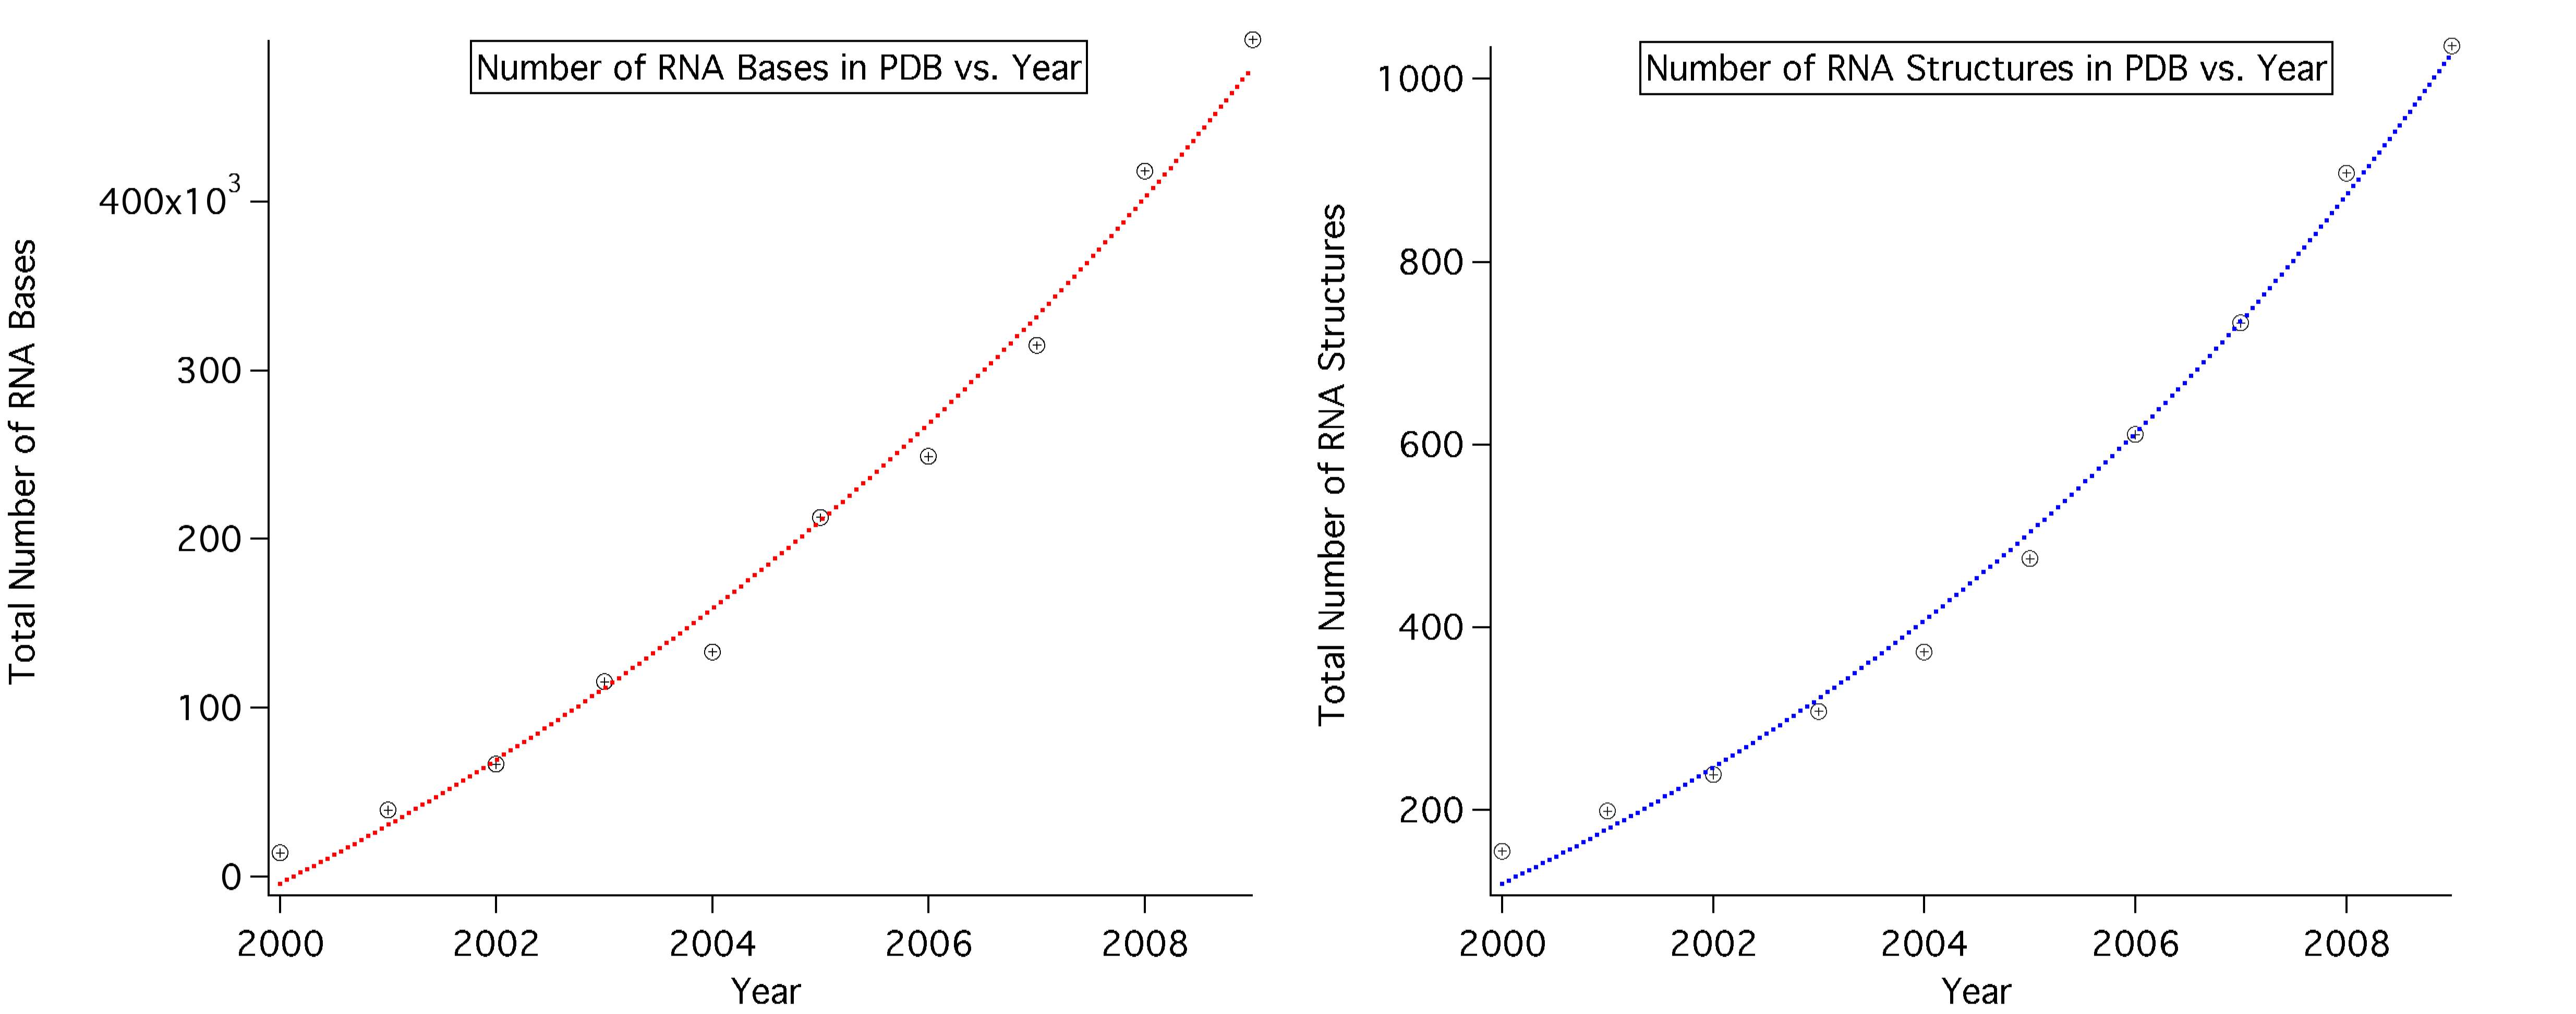
\includegraphics[scale=0.38]{Chapter2/rna2000_2009copy.png}
\caption{\textbf{Right:} Total  number of RNA  bases added to  the PDB
database  between 2000 and  2010 (Exponential fit line in
blue). \textbf{Left:}  Total number  of RNA structures  solved yearly
by X-Ray  crystallography between  2000 and 2010 (Exponential fit line
in red).}
\label{fig:rnainpdb}
\end{figure}

\noindent Between  1978 and  2000 a total  of 116 RNA  structures with
resolution greater than 3.5\AA,  and comprising around 5500 nucleotide
bases are found  in the Protein Data Bank (PDB),  and between 2000 and
today  a  total of  931  RNA\index{RNA}  structures comprising  491158
nucleotide bases are found.  That  is, the increase in information due
to  the  solution of  large  RNA structures  is  about  two orders  of
magnitude as pointed out  by Noller \cite{noller2005}.  Looking at the
growth  of RNA  structural information  from 2000  until today,  it is
clear that  both the total number  of RNA structures  deposited to the
PDB, and the total number  of nucleotide bases in these structures, is
growing in an exponential way (as  can be seen by the exponential fits
in  Figure~\ref{fig:rnainpdb}).   It's  important  to note  that  such
growth comes mainly from ribosomal structures which contain 88 percent
of all RNA  bases in the PDB.  So, even  though structural interest in
RNA is  growing since ribosomal  structures became available  in 2000,
and several  Nobel prizes  have been awarded  for work in  this field,
along  with  the  exciting  possibilities  of  deciphering  large  RNA
\cite{weinberg2009}  structures  other than  the  ribosome, still  the
growth of  the RNA structural  field is far  from that of  proteins if
weighed by  the growth in  diversity of RNA structural  information in
the past decade. At the present time if we look at the distribution of
RNA  sizes   counted  by   number  of  bases,   as  can  be   seen  in
Figure~\ref{fig:rnaranges}  it's clear  that there  are  great patches
where there are no RNA  structures whatsoever, roughly between 600 and
1400 bases  and between  1800 and 2700  bases. The area  of non-coding
RNA's holds great promise for  finding structured RNA's in such length
ranges    as    has     recently    been    suggested    by    Breaker
\cite{weinberg2009}.  A representative  example of  the characteristic
ranges of RNA  structures available to date in the PDB  can be seen in
Table~\ref{tab:rnarange}  for structures  larger than  300  bases.  An
interesting comparison between the  total number of structures of RNA,
protein, dna, and nucleic acid plus protein, available at the PDB from
the   seventies    until   today    can   be   seen    in   Supplement
Figure~\ref{fig:allpolypdb}.

\begin{figure}[H]
\centering
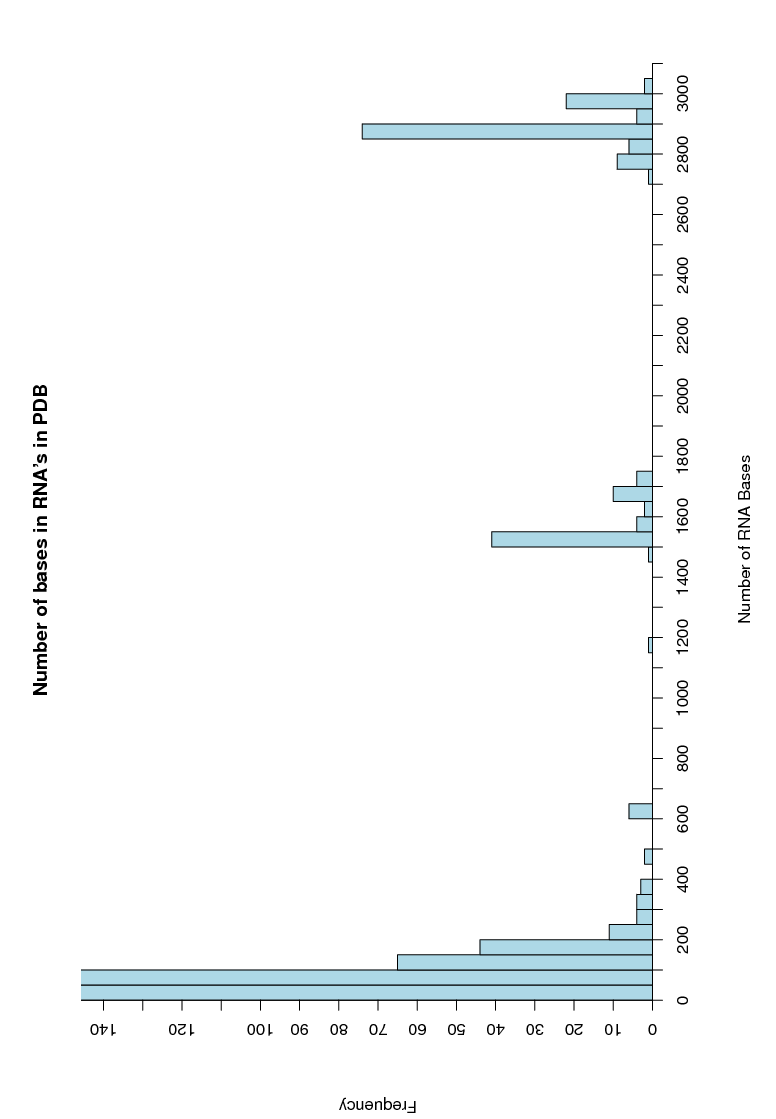
\includegraphics[scale=0.60, angle=270]{Chapter2/histogram.png}
\caption{Frequency of nucleotide bases in RNA molecules found in the
  PDB classified by the size of RNA molecules. We define the size as the
  total number of nucleotide bases present per molecule.}
  \label{fig:rnaranges}
\end{figure}
%The table and Figure 1.1 come from downloading all structures from
%2000, until today that have RNA in the pdb and that have a resolution
%better that 3.0A, they are 460 structures.

\noindent The analysis of  RNA conformational information contained in
RNA structural  data can be  divided into three main  perspectives: an
atom based perspective; a bond  based perspective; and a third, as yet
unexplored  to our  knowledge, rigid-body  based perspective.   In the
atom  based perspective,  either  direct comparison  of backbone  atom
positions is  made \cite{reijmers2001},  or a comparison  of distances
between a  reduced set  of atoms taken  from the  nucleotide backbone,
sugar,  and  base \cite{sykes2005}.   The  bond  based perspective  is
divided  into   three  main   categories;  the  first   considers  the
consecutive covalent bonds in the RNA backbone and the glycosidic bond
between the sugar  and base, that is, six  backbone torsion angles and
one   glycosidic   torsion   angle   \cite{reijmers2001,   murray2003,
  hershkovitz2003,  schneider2004, hershkovitz2006};  or alternatively
the  pseudo-bonds between consecutive  P and  C4$^{\rm{\prime}}$ atoms
and   the  resulting   pseudo-torsion  angles   $\eta$   and  $\theta$
\cite{olson1_1972,               duarte1998,               duarte2003,
  wadley2007} \footnote{Previously the pseudotorsion angles $\eta$ and
  $\theta$    were    given     the    names    $\omega_{\nu}$,    and
  $\omega_{\nu\rm{\prime}}$.\cite{malathi1985}}.   The  third category
considers the networks of  horizontal hydrogen bonding patterns coming
from  a definition of  interacting edge  boundaries in  the nucleotide
bases \cite{westhof2000, leontis2002, leontis2006}. In this chapter we
study the rigid body based perspective using clustering analysis.
\begin{table}[htbp]
\begin{center}
{\small
\begin{tabular}{c|p{5cm}|c|c|c}
\hline
\bf{PDBID} & \bf{Structure Name} & \bf{Phylogenetic Group} & \bf{Number of bases} & \bf{Year} \\ \hline
1l8v & Mutant of P4-P6 Domain of Group I Intron & Eukaryote & 314 & 2002 \\ \hline
3igi & Group II Intron & Bacteria & 395 & 2009 \\ \hline
1fg0 & Central Loop in Domain V of 23S rRNA & Archaea & 499 & 2000 \\ \hline
2nz4 & GlmS Ribozyme & Eukaryote & 604 & 2006 \\ \hline
1xmq & 30S rRNA & Bacteria & 1522 & 2004 \\ \hline
1ffk & 50S rRNA Subunit & Archaea & 2828 & 2000 \\ \hline
\end{tabular}
}
\caption{Some large RNA structures ($>$300 bases) elucidated in the last decade.}
\end{center}
\label{tab:rnarange}
\end{table}

\section{Consensus Clustering of Single Stranded Base Step Parameters}
To  our  knowledge there  has  been  no  classification of  rigid-body
base-step parameters  for RNA structures  deposited at the PDB.  It is
important  to note  here that  in  crystal structures,  RNA bases  are
determined more  accurately than backbone torsion angles,  as has been
shown by Richardson  and collaborators from analysis of  van der Waals
steric    clashes.    This    can    be   seen    more   clearly    in
Figure~\ref{fig:murray},    reproduced    from    Richardson's    work
\cite{murray2003}, where the red and orange dots in the backbone atoms
region denote steric clashes and the green and yellow dots in the base
atoms region  denote very good  agreement with expected van  der Waals
distances.
\begin{figure}[htbp]
 \centering
 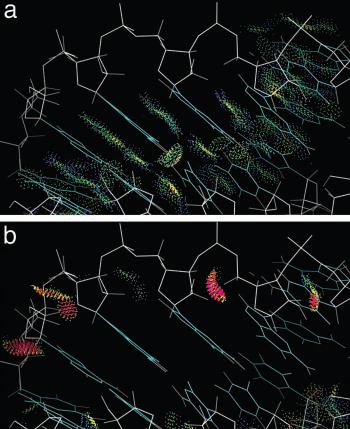
\includegraphics[scale=0.5]{Chapter2/murray2003.png}
 \caption{Figure taken from  Richardson et al. \cite{murray2003} where
 the  blue and  green dots  in  a) mean  very accurate  van der  Waals
 distances, and  in b)  the red and  orange dots mean  steric clashes,
 that is, distances outside the acceptable van der Waals range.}
 \label{fig:murray}
\end{figure}

\subsection{Combining Fourier Averaging Results and Clustering Analysis}
Using  the  coordinate  files  of  20  rRNA  structures  provided  by
Schneider  at  al.\cite{schneider2004}  we  used  standard  clustering
analysis  (CA)  techniques (see  Appendix  A)  to  classify a  set  of
non-ARNA base-steps using, rather  than the more common torsion angles
space, the  base-step parameters  space, that is,  three translational
parameters  (Shift   $D_x$,  Slide  $D_y$,  Rise   $D_z$),  and  three
rotational  parameters  (Tilt $\tau$,  Roll  $\rho$, Twist  $\omega$),
which we describe with the hexaparametric vector $\nu$:
\begin{gather}
 \nu = (D_x, D_y, D_z, \tau, \rho, \omega)
\end{gather}
The results illustrated in Figures~\ref{fig:eucl_cons} ~\ref{fig:steps2}
and~\ref{fig:nonAclus} were obtained by performing clustering analysis
and consensus clustering on 20 structures provided by Schneider et al.
\cite{schneider2004}.   These  twenty   structures  were  obtained  by
Schneider applying a  Fourier averaging technique, and lexicographical
clustering, to  torsion angles of  23S rRNA.  The methodology  we used
follows   that  used  by   others  to   recover  the   periodic  table
classification  from multidimensional  property  vectors for  elements
\cite{restrepo2004, restrepo2006}.
\begin{figure}[htbp]
 \centering
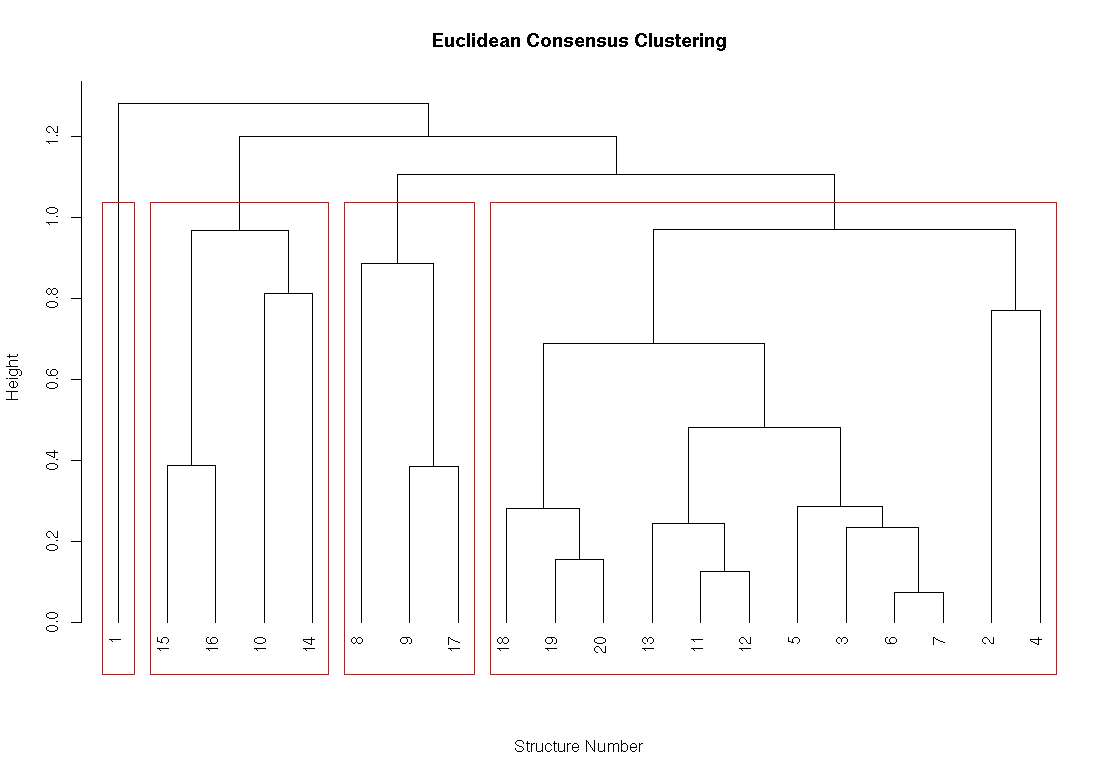
\includegraphics[angle=90, scale=0.6]{Chapter2/eucli_cons_nonA-RNA.png}
\caption{Dendrogram showing the results  of consensus clustering of 20
non-Atype  rRNA  dinucleotides   according  to  their  hexadimensional
base-step parameter vectors.}
 \label{fig:eucl_cons}
\end{figure}

\begin{figure}[htbp]
 \centering
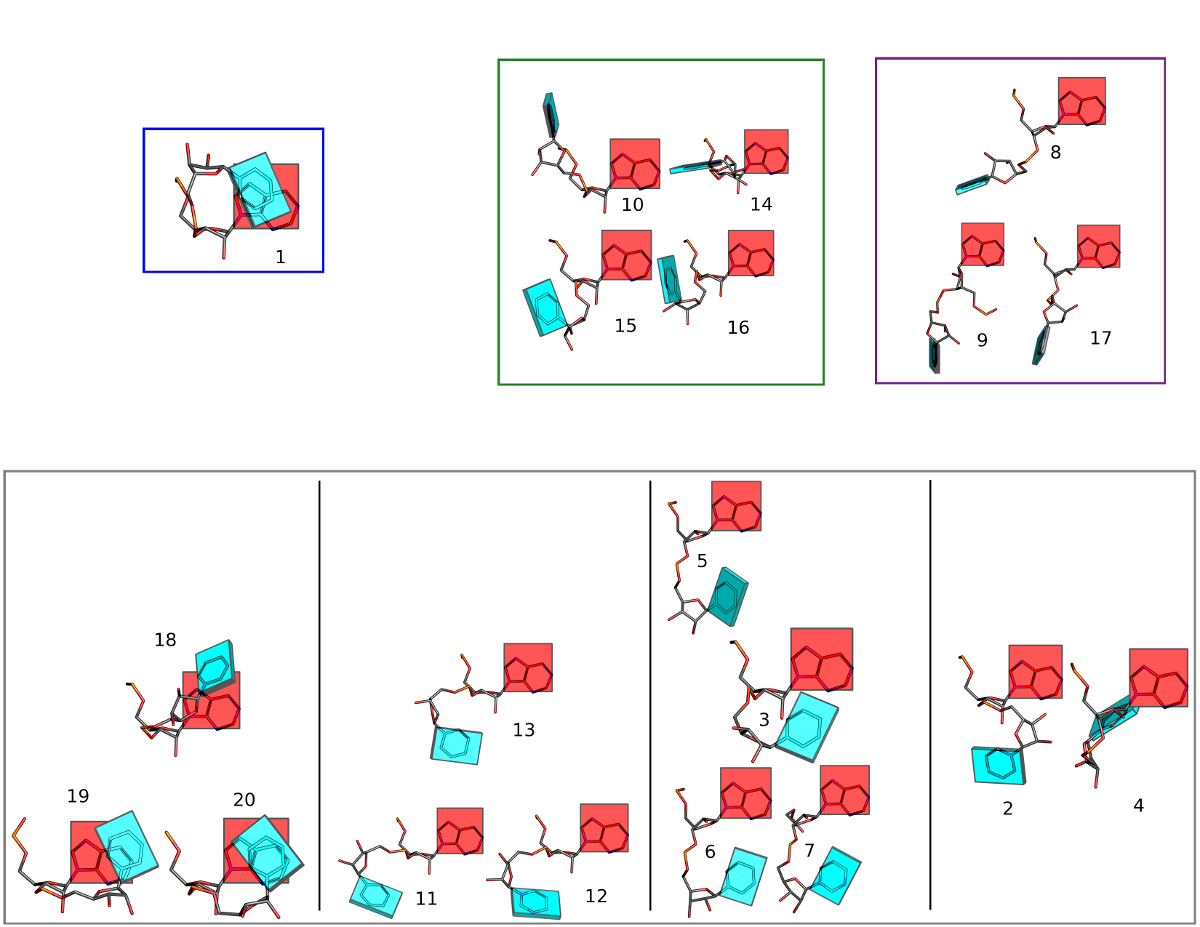
\includegraphics[angle=90, scale=0.5]{Chapter2/collageb.png}
 \caption{rRNA dinucleotide structures organized by clusters obtained from
consensus clustering of their hexadimensional base-step parameter vectors.}
 \label{fig:nonAclus}
\end{figure}

Group I  contains a single structure {1}  with base-plane normals
pointing   in  opposite   directions,  Group   II   includes  extended
conformations with neighboring bases  roughly parallel but not stacked
and is formed by structures {15,  16, 10, 14}, Group III also contains
extended conformations with bases  perpendicular to one another and is
formed by structures {8, 9, 17}, Group  IV {18, 19, 20, 13, 11, 12, 5,
  3, 6, 7, 2, 4} contains  four major subgroups: (a) structures {2, 4}
which are unstacked with bases neither parallel nor perpendicular; (b)
structures {18, 19,  20} which closely related to A-RNA; (c) structures {11,
  12,  13}  which are  unstacked  and  have  parallel bases;  and  (d)
structures {3,  5, 6,  7} which are  also unstacked and  have parallel
bases. We also see in Group IV that the conformers in subgroups IV (c)
and  IV (d)  are closely  related  and that  the dimers  in these  two
subgroups are more closely related to those in subgroup IV (b) than to
those in subgroup IV (a).


When looking at Table~\ref{tab:nonA}, it's clear that there are 1858
steps (67\%) which are not classified into any of the groups. The reason for
this is the mixing of Fourier averaging for backbones, and the
base step perspective. It might also be that we are not using the
other A-RNA like backbone based structures from schneider's paper.

Right now I am doing a validation with clValid, to see if anything
pops up regarding the "optimal" number of clusters for the data.
Perhaps it would be wise to filter the data by proximity to A-RNA like
conformation, say, take all structures which are some RMSD, or
manhattan, or euclidean distance appart from the cannonical A-RNA step
parameters which are in table such and such.


Table~\ref{tab:nonA}  shows  the
residue  numbers of  bases  from 23S  rRNA  which belong  to the  main
categories of Figure~\ref{fig:nonAclus}.   To match residues of
23S  rRNA belonging  to the  non-Atype  clusters, a  root mean  squared
deviation (RMSD)  of 15  or less was  required between  step parameter
vectors  of 23S  rRNA  and the  mean  parameter vectors  for the  four
non-Atype groups identified.
\begin{table}[htbp]
\begin{center}
{\footnotesize
\begin{tabular}{p{3cm}|p{1,3cm}|c|c|p{3cm}|p{3cm}}
\hline
\bf{Total Number of Nucleotides} & \bf{RMSD Limit} & \bf{Group}
& \bf{Base-steps} & \bf{Base-step Residue Number}
& \bf{Overlaps} \\ \hline
2754 & $ < 15$ & I & 3 & 892, 2006, 2390 &  \\ \hline
 &  & II & 5 & 459, 1279, 1653, 1919, 2302 &  \\ \hline
 &  & III & 1 & 2109 &  \\ \hline
 &  & IV & 35 & 79, 112, 128, 190, 213, 269, 358, 434, 488, 564, 706,
 720, 775, 867, 966, 1292, 1503, 1543, 1614, 1766, 1874, 1908,
 1971, 2017, 2257, 2427, 2516, 2540, 2755, 2782, 2810, 2826,
 2874, 2882, 2913 &  \\ \hline
 &  & IVa & 1 & 882 &  \\ \hline
 &  & IVb & 807 &  &  \\ \hline
 &  & IVc & 9 & 306, 789, 854, 880, 1107, 1192, 1493, 1818, 2005 &  \\ \hline
 &  & IVd & 35 & 175, 213, 246, 264, 304, 358, 464, 518, 531, 534,
 588, 795, 938, 1214, 1231, 1316, 1340, 1370, 1605, 1745, 1766, 
 1971, 1976, 2010, 2017, 2291, 2320, 2428, 2469, 2481, 2516, 2532, 
 2755, 2826, 2882 & Only IVd with IV (213, 358, 1766, 1971, 2017, 
 2516, 2755, 2826, 2882) \\ \hline
\end{tabular}
}
\caption{Residue numbers for base-steps  with RMSD values less than 15
between  the  reference base-step  vectors  from  the  four groups  of
non-A-type  RNA dinucleotide conformations  and all  base-step vectors
found  in  the 23S  strand  of  \textit{Haloarcula marismortui}  large
ribosomal subunit.}
\label{tab:nonA}
\end{center}
\end{table}



%%%%%%%%%%%%%%%%%%%%%%%%%%%%%%%%%%%%%%%%%%%%%%%%%%%%%%%%%%%%%%%%%%%%%%
%
% INCLUDE HERE PICTURES OF POSITIONING OF NON-ARNA GROUPS IN
% RIBOSOME.
%
%%%%%%%%%%%%%%%%%%%%%%%%%%%%%%%%%%%%%%%%%%%%%%%%%%%%%%%%%%%%%%%%%%%%%%


\subsection{Partitional Clustering for Rigid Body Parameters}
The argument I thought could have been made was that with clustering
analysis alone on the whole data set, the A-RNA data would split
naturally, without recurring to other ideas like Fourier Filtering of
Bergman et al.

We also analyze the 2753 base-step parameter vectors in the ribosome.
For the partitional clustering case,
again, there  is no known  number of clusters  in which the  data must
group, therefore  we've calculated the within clusters  sum of squares
and also the average silhouette  widths, for a particular selection of
the  number   of  partitions  of   the  data  for   $k=[2-80]$.   From
figure~\ref{fig:wssSteps}  we can't  conclude  much. We  see that  the
value of  the within clusters  sum of squares becomes  constant around
$k=47$ and there´s also a  change of curvature around $k=13$.  For the
case where  the average  silhoutte width has  been computed,  that is,
figure~\ref{fig:aswSteps}, we  see that the maximum is  for $k=2$, and
there are  some interesting  maxima at $k=9,12$.   Now that we  have a
clue as to  which number of partitions the data  optimally has we have
plotted the  k-means results for  $k=13$ and $k=47$ in  Figures number
and number, and the PAM results for $k=2, 9, 12$ in Figure number.

We have also  filtered the data according to the  16 possible RNA base
steps, that is,  AA, AG, GA, GG, UU,  UC, CU, CC, UA, UG,  CA, CG, AU,
AC, GU, and  GC.  Tables showing how many  representatives steps there
are belonging to non-helical,  helical, and watson-crick sets, will be
later included and discussed here.
\begin{figure}[htbp]
\centering
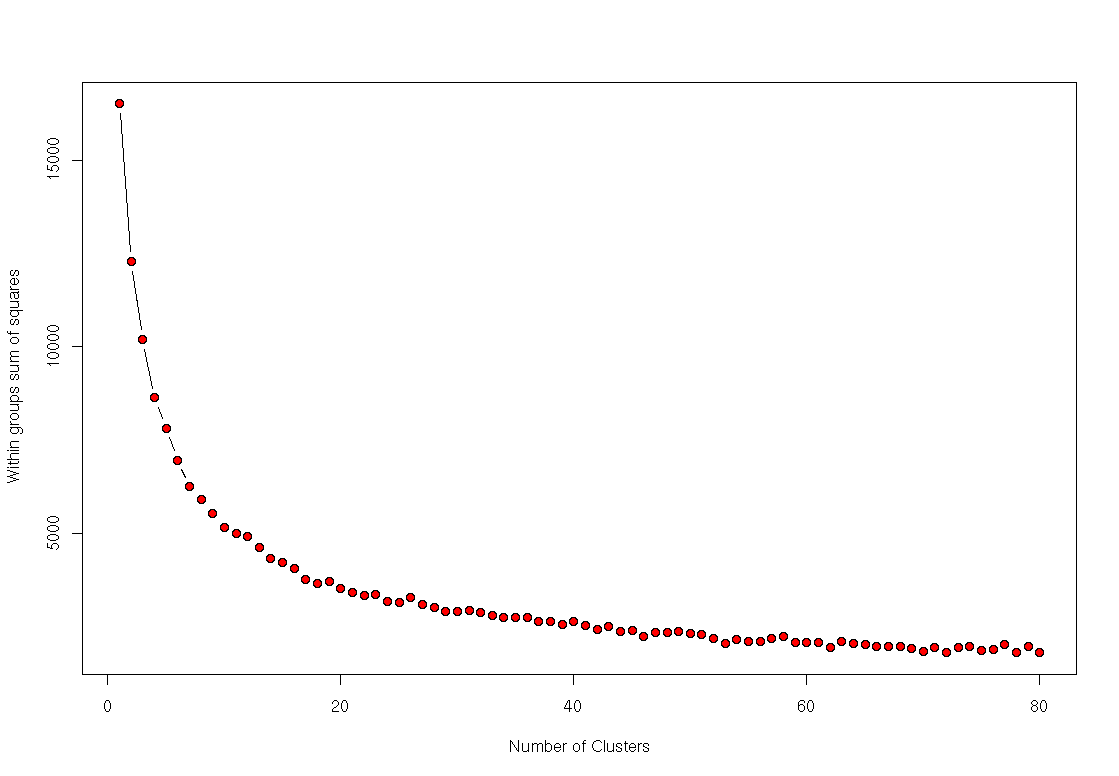
\includegraphics[angle=0, scale=0.40]{Chapter2/hartigan_nuclu_steps_b.png}
\caption{Sum of all within clusters sum of squares against number of clusters.}
\label{fig:wssSteps}
\end{figure}

\begin{figure}[htbp]
 \centering
 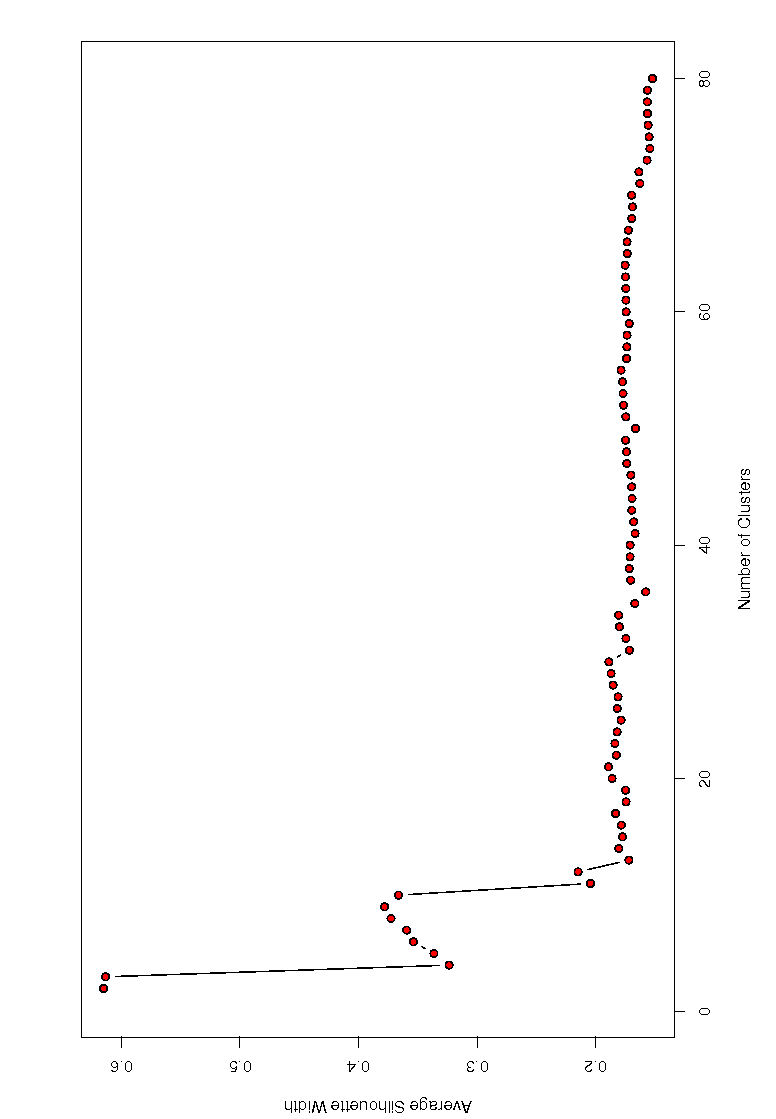
\includegraphics[angle=270, scale=0.50]{Chapter2/pam_asw_2_80_steps.png}
 \caption{Average silhouette width against number of clusters.}
 \label{fig:aswSteps}
\end{figure}



\subsection{Hierarchical Clustering for Rigid Body Parameters}

Also as has been carried out for torsion angles, hierarchical clustering has
also been performed on rigid body parameters, the results are yet to be
included here. A cluster dissimilarity tree can be seen in
Figure~\ref{fig:clusdis} for the 12 trees resulting from the four clustering
methods and three distance definitions used to cluster the base step data.

\begin{figure}[htbp]
\centering
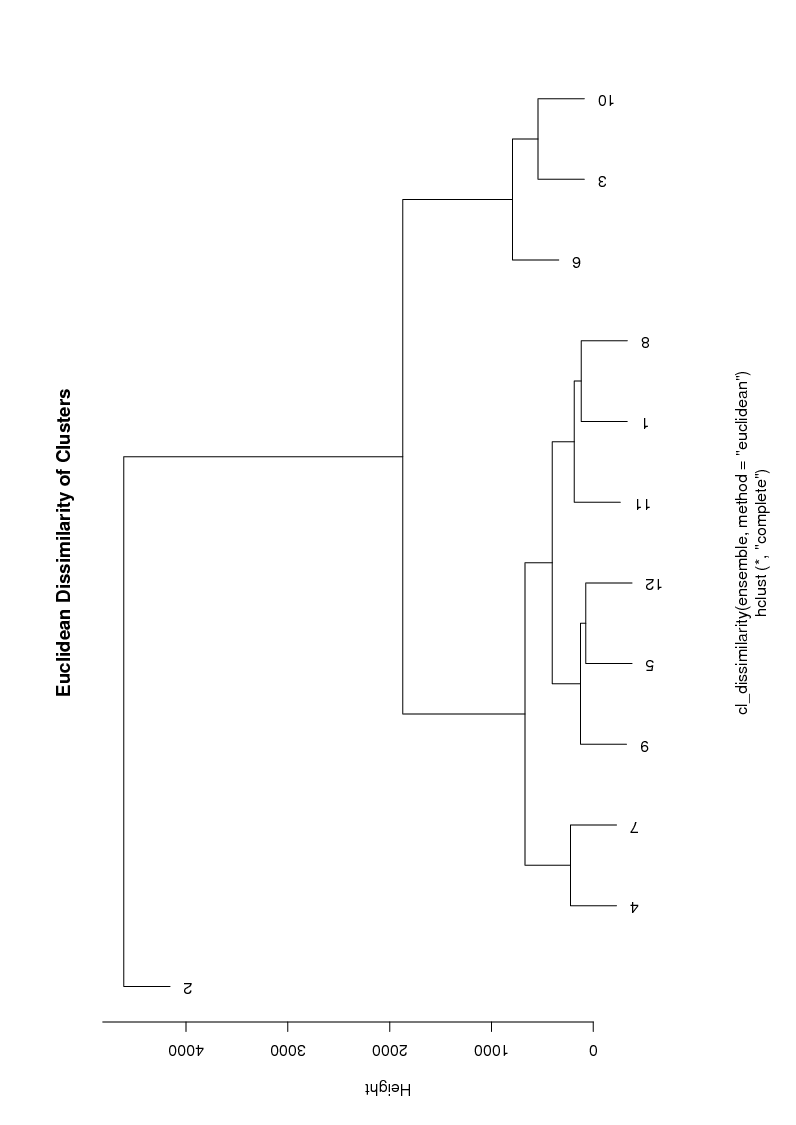
\includegraphics[scale=0.60]{Chapter2/clussdissim.png}
\caption{Cluster dissimilarities for the twelve hierarchical trees
  obtained from clustering of the six-dimensional base-step parameters
obtained from the large subunit of the ribosome (PDB-ID:1jj2)}
\label{fig:clusdis}
\end{figure}


\section{RNA Conformations}
There are two main RNA conformations, A-RNA ,and A'RNA, and maybe even a
third unconfirmed one A"RNA \cite{saenger1984}.
Their values for their standard torsion angles and step parameters can be seen
in Tables~\ref{tab:tor_conf} and ~\ref{tab:step_conf} 

\begin{table}[htbp]
\begin{center}
{\small
\begin{tabular}{c|c|c|c|c|c|c|c|c}
\hline
\bf{Structure Name} & $\alpha$ & $\beta$ & $\gamma$ & $\delta$ & $\epsilon$
& $\zeta$ & $\chi$ & \bf{Reference} \\ \hline
A-RNA & -68.9 & 179.5 & 54.5 & 82.2 & -153.9 & -70.8 & -161.1 & Arnott \\ \hline
A'-RNA & -70.0 & 176.6 & 60.8 & 76.7 & -153.4 & -69.4 & -163.4 & Arnott \\ \hline
AII-RNA & -65.0 & 175.1 & 52.9 & 81.1 & -166.0 & -68.0 & -157.0 & Schneider \\ \hline
\end{tabular}
}
\caption{Base step torsion angles for the different known RNA conformations.}
\label{tab:tor_conf}
\end{center}
\end{table}

\begin{table}[htbp]
\begin{center}
{\small
\begin{tabular}{p{2cm}|c|c|c|c|c|c|c}
\hline
\bf{Structure Name} & Shift ($D_x$) & Slide ($D_y$) & Rise ($D_z$) & Tilt
($\tau$) & Roll ($\rho$) & Twist ($\Omega$) & \bf{Reference} \\ \hline
A-DNA & 0.36 & -1.39 & 3.29 & 2.46 & 12.50 & 30.19 & \\ \hline
B-DNA & 0.44 & 0.47 & 3.33 & 4.63 & 1.77 & 35.67 & \\ \hline
A-RNA & -0.08 & -1.48 & 3.30 & -0.43 & 8.64 & 31.57 & Arnott \\ \hline
A'-RNA & 0.05 & -1.88 & 3.39 & -0.12 & 5.43 & 29.52 & Arnott \\ \hline
AII-RNA & 1.01 & -2.52 & 3.33 & 2.94 & 9.75 & 25.12 & Schneider \\ \hline
\end{tabular}
}
\caption{Base step parameters for the different known RNA
  conformations. Notice that the base step parameters are for single
  bases rather than base-pairs.}
\label{tab:step_conf}
\end{center}
\end{table}




\begin{figure}[htbp]
\centering
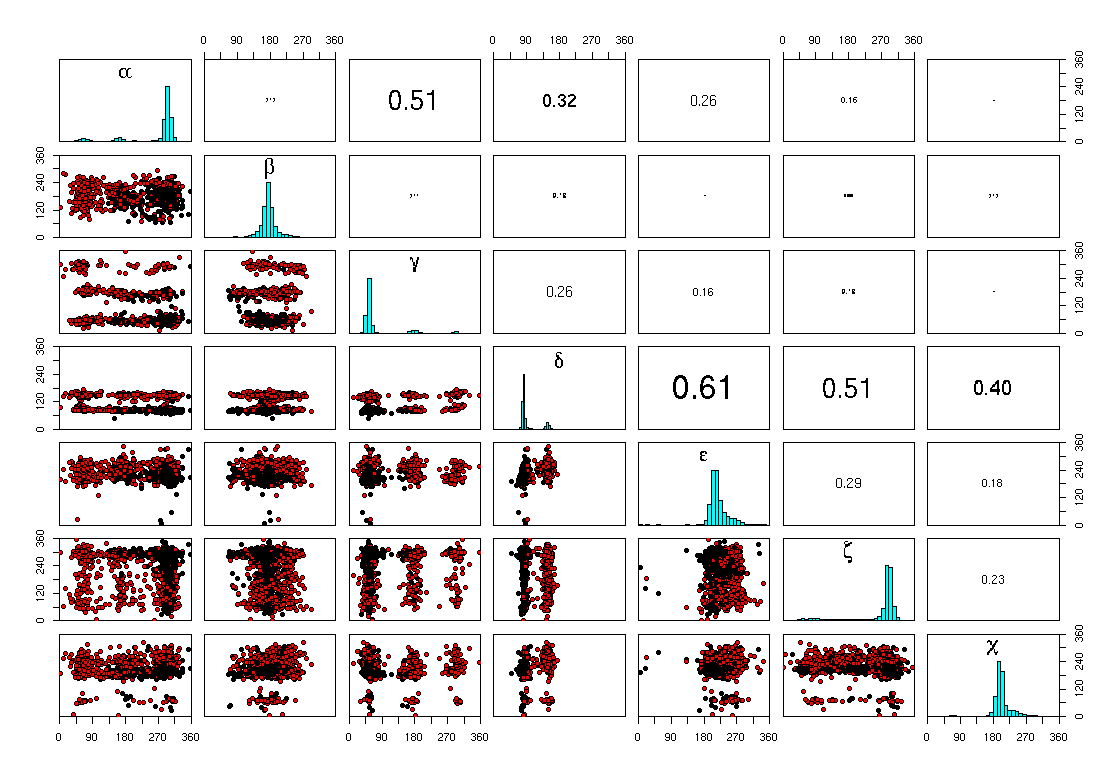
\includegraphics[angle=90, scale=0.50]{Chapter2/hartigan_tor_b.png}
\caption{
K-means of torsion  angle vectors of 2753 dinucleotide steps
present in  23S rRNA using the  \textit{Hartigan-Wong} algorithm.  The
number  of  partitions  is  \textbf{2}.   The  upper  diagonal  matrix
displays the values  of the linear correlation coefficient  $r$, and a
histogram showing  the torsion angle distribution is rendered  in the
diagonal.}
\label{fig:hartigan}
\end{figure}

\begin{figure}[htbp]
\centering
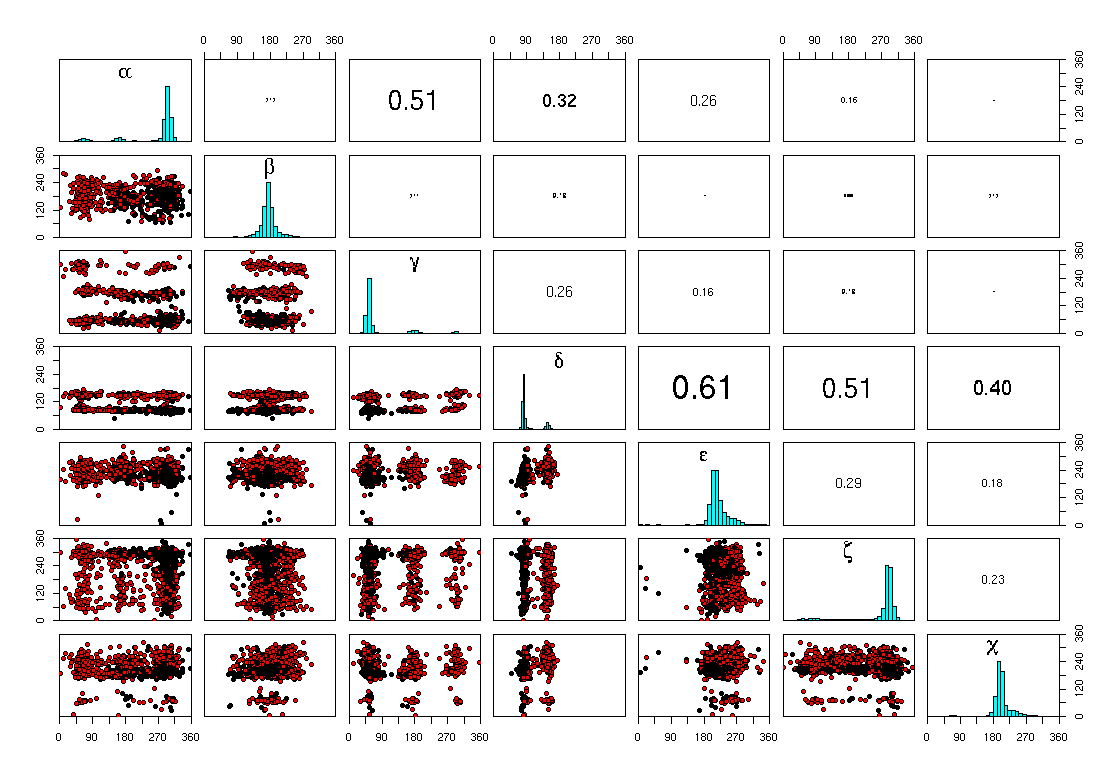
\includegraphics[angle=90, scale=0.50]{Chapter2/lloyd_tor_b.png}
\caption{
K-means of torsion  angle vectors of 2753 dinucleotide steps
present in  23S rRNA using the  \textit{Lloyd} algorithm.  The
number  of  partitions  is  \textbf{2}.   The  upper  diagonal  matrix
displays the values  of the linear correlation coefficient  $r$, and a
histogram showing  the torsion angle  distribution is rendered  in the
diagonal.}
\end{figure}

\begin{figure}[htbp]
\centering
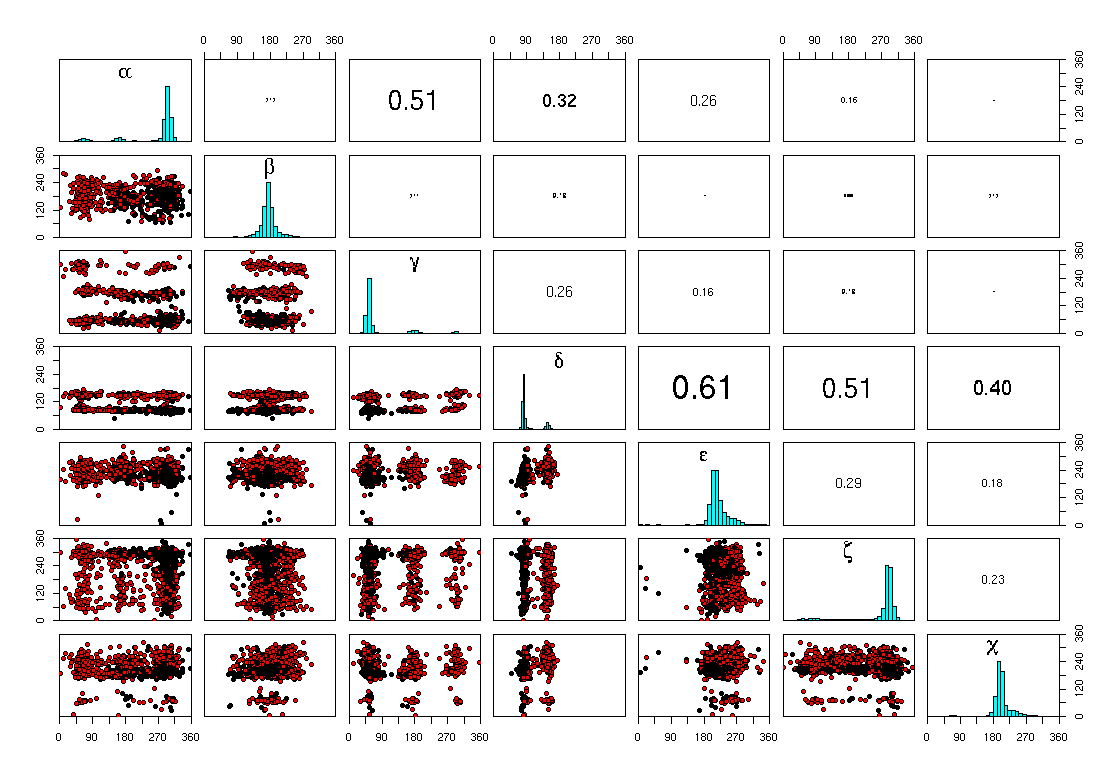
\includegraphics[angle=90, scale=0.50]{Chapter2/forgy_tor_b.png}
\caption{
K-means of torsion  angle vectors of 2753 dinucleotide steps
present in  23S rRNA using the  \textit{Forgy} algorithm.  The
number  of  partitions  is  \textbf{2}.   The  upper  diagonal  matrix
displays the values  of the linear correlation coefficient  $r$, and a
histogram showing  the torsion angle  distribution is rendered  in the
diagonal.}
\end{figure}

\begin{figure}[htbp]
\centering
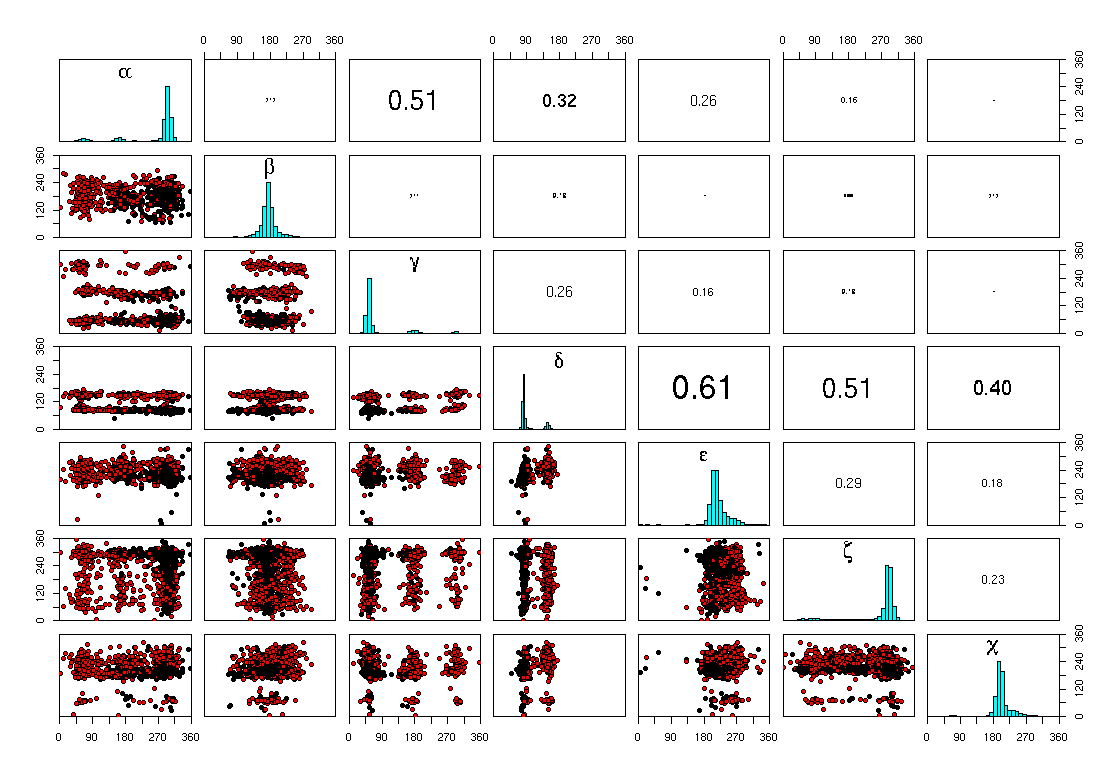
\includegraphics[angle=90, scale=0.50]{Chapter2/macqueen_tor_b.png}
\caption{
K-means of torsion  angle vectors of 2753 dinucleotide steps
present in  23S rRNA using the  \textit{McQueen} algorithm.  The
number  of  partitions  is  \textbf{2}.   The  upper  diagonal  matrix
displays the values  of the linear correlation coefficient  $r$, and a
histogram showing  the torsion angle  distribution is rendered  in the
diagonal.}
\label{fig:macqueen}
\end{figure}




\bibliography{biblio}

